\documentclass[conference]{IEEEtran}
\IEEEoverridecommandlockouts
% The preceding line is only needed to identify funding in the first footnote. If that is unneeded, please comment it out.
\usepackage{cite}
\usepackage{amsmath,amssymb,amsfonts}
\usepackage{algorithmic}
\usepackage{graphicx}
\usepackage{textcomp}
\usepackage{xcolor}
\def\BibTeX{{\rm B\kern-.05em{\sc i\kern-.025em b}\kern-.08em
    T\kern-.1667em\lower.7ex\hbox{E}\kern-.125emX}}
\begin{document}

\title{Implementation and verification of a data vault\\\Large Storing and Managing Data (Module 06-32245), Autumn 2022}

\author{\IEEEauthorblockN{Surname, Name, Student ID}
abc123@student.bham.ac.uk\\
\today}


\maketitle

\begin{abstract}
As the adoption of technology increases and companies continue to expand their business in this sphere, the amount of data generated by users will only grow. However, the data collected is heterogeneous and has to be converted into organised information that forms the basis of reporting and aids in decision-making. Data vault illustrates the implementations and steps to gather data from multiple sources and make it available in the form of a unified information store to serve clients needs. Data vaults allow the agile development approach to build an enterprise warehouse that is capable of historical data tracking and enables auditing. This is implemented in tiers of staging, enterprise data warehouses and information marts. Instead of focusing on a single topic for analysis, an enterprise data warehouse aims to represent all of the business data and business rules of an organisation. Information in the warehouse is presented so that business users can access all pertinent subject areas from individual information marts that contains a subset of the information kept by the business in a larger storage system.
\end{abstract}

\section{Introduction}\label{sec:Intro}
Any organisation now considers the information to be a valuable resource to be able to make informed decisions and contribute value to the organisation. Data vault ``Fig.~\ref{fig1}'' enables them to achieve this goal for multiple use cases across the organisation. Every function or department has various demands for the data to be studied, so the enterprise data warehouse must offer a variety of subject areas to satisfy those needs.


\begin{figure}[htbp]
\centerline{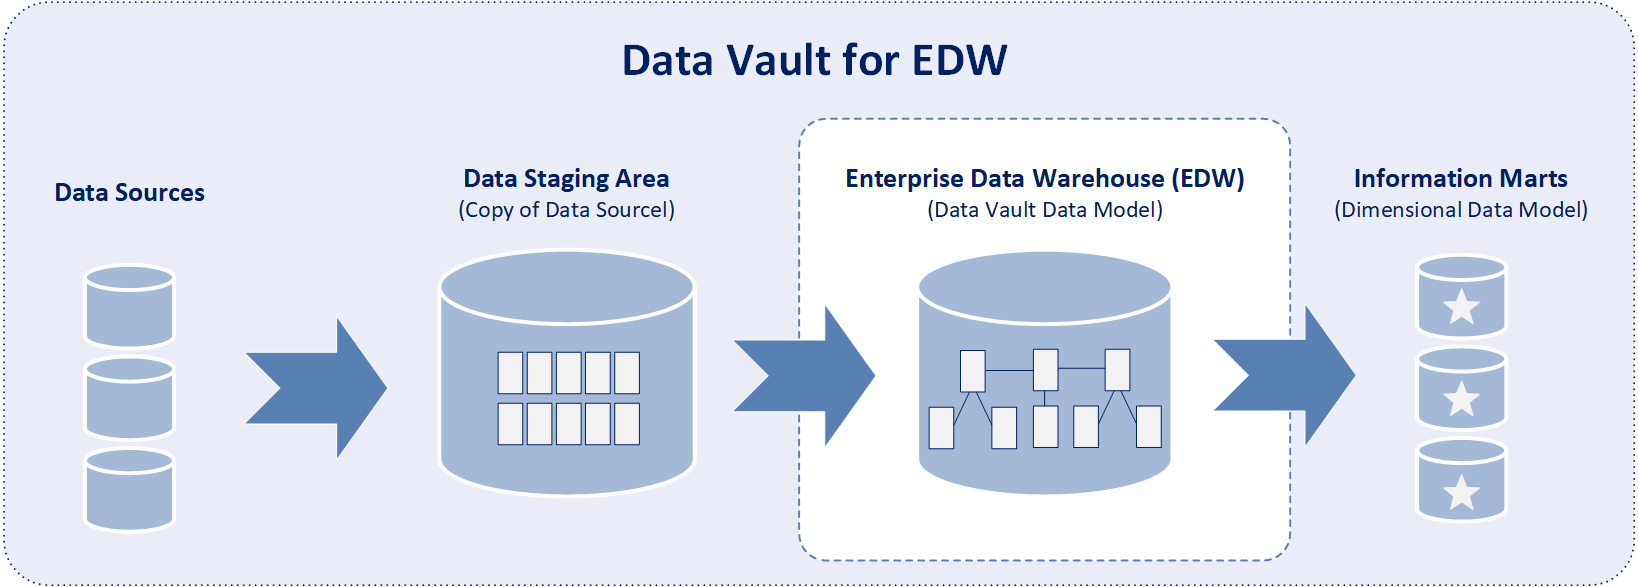
\includegraphics[width=9cm, height=4cm]{Figure1.png}}
\caption{Data Vault Schemata}
\label{fig1}
\end{figure}

Data vault is implemented with a three-tier architecture made up of \textbf{Staging}, \textbf{Enterprise Data Warehouse} and \textbf{Information Marts}.

\subsection{Staging Layer}

Before the data is imported to enterprise warehouses, the staging layer is a place for loading and processing of source data. The staging area is used to aggregate data from various source systems and undergo transformations once data has been placed into it. At the staging area, ETL processing is executed.

\smallskip
\noindent ETL Process is divided into three steps:

\begin{enumerate}
\item Extract
\item Transform
\item Load
\end{enumerate}

\textbf{Extract} comprises gathering the information from various data sources that will be used to populate the data warehouse.

\textbf{Transform} receives data from extract stage and makes data ready to load in enterprise data warehouse. In data vault, data are segregated into Hubs, Links and Satellites. The data received is logically divided into pieces suitable to load according to enterprise entities. Therefore, each section of data will be divided during the transform step and then reorganised into a format consistent with the database design.

\textbf{Load} receives transformed data to be inserted into data vault. 

Business key, the identity of the person inserting the data, is added to the source during ETL process together with current timestamp.

\subsection{Enterprise Data Warehouse Layer}

Data warehouse model ``Fig.~\ref{fig2}'' represents business processes and is tied to business through business keys. With the orientation of data vault model on business keys, we inherit the ability to integrate, connect and access information in the same manner as the business does in its daily operations \cite{b1}.

\begin{figure}[htbp]
\centerline{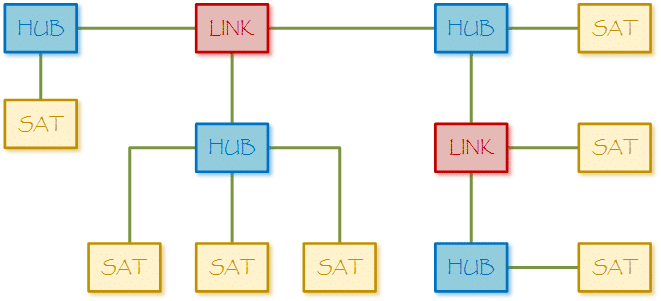
\includegraphics[width=9cm, height=4cm]{Figure2.png}}
\caption{Enterprise Data Warehouse Components}
\label{fig2}
\end{figure}

\smallskip
\noindent A data vault architecture is comprised of three main structures:

\begin{enumerate}
\item Hub
\item Link
\item Satellite
\end{enumerate}

A distinct set of business keys that describe fundamental business concepts acts as a \textbf{hub}. These distinct business keys are required to identify the information and business users use them to refer to a business object when requesting information from an operational system. There are hubs for each area of business information.

Each business object interacts with others in some way. They are linked together by the operational business processes, which employ business objects to carry out their functions. These connections are modelled by the Data Vault using a \textbf{link} that join two or more hubs.

A \textbf{satellite} is a table with extensive descriptive data that places the business keys from the Hub or Link in proper perspective. Whenever changes to the data warehouse's descriptive data occur, it collects them with a new timestamp that represents a newer version.

\subsection{Information Mart layer}

Data vault modeling is unfamiliar to a majority of business customers. In order to obtain useful and usable data that can be utilised for processing into actionable information, they also need to be able to grasp how to combine the numerous entities. An information mart ``Fig.~\ref{fig3}'' is often used by end users to obtain prepared information that they can immediately utilise for the task at hand. As a means of user services, this layer queries from the enterprise layer. Information marts are designed in start schema each of which exposes a portion of the vault for a certain user group. Hubs and their satellites often create dimensions, whereas links and their satellites create facts.

\begin{figure}[htbp]
\centerline{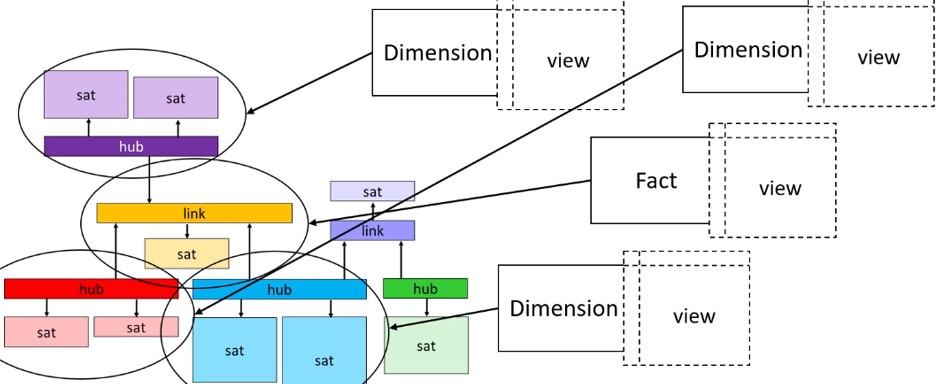
\includegraphics[width=9cm, height=4cm]{Figure3.png}}
\caption{Virtualized Information Mart}
\label{fig3}
\end{figure}


\section{State of the art of data vaults}

The need for easy access to organised storage of high-quality data for decision-making prompted the concept of data warehousing. Organizations hold huge amounts of data, but accessing and utilising it has become increasingly difficult and complex as a result of the information being available in a number of forms and sitting in a variety of file and database structures. Building a data warehouse requires a modeling approach that considers all aspects of development such as data modeling, project management, risk management, deployment and many other essential aspects \cite{b2}.

There were several approaches made to address them, \textbf{Bill Inmon} in 90's approached by creating a central repository that stores data in a database, the database is divided into separate layers. Data marts and data warehouse are considered separate physical structures. In this model, data marts are loaded from the same data warehouse, so they remain consistent. Issues arise as the requirements increase, this model becomes complex and requires more tables, querying this database also becomes complex as it involves more joins. \textbf{Kimball} during the 90's proposed a new dimensional architecture. He proposes data warehouse itself can be considered a form of data mart consisting of fact Tables and dimension tables. This approach would have fewer joins since the dimension tables are denormalized, but we see update anomalies and redundant data being stored.

The Enterprise Data Warehouse design have evolved thanks to the Data Vault data model proposed by \textbf{Linstedt} as an alternative to Inmon's and Kimball's traditional data warehouse architecture's. According to Linstedt, the 3NF of Inmon and the dimensional modeling of Kimball have weaknesses if the data volume increases \cite{b3}. Dan Linstedt defines the Data Vault as “a detail-oriented, historical tracking and uniquely linked set of normalized tables that support one or more functional areas of business”.

\section{Methods}

Raw data is received from multiple domains having different source systems, Initially, the data is read from the source systems and put in a staging area. A python program reads the data repository and collects information in raw format. It reads the metadata and stores it in a dictionary. Each of the dictionary values represents a key, value pair. Then the data is read in a two-dimensional array format. The next step in staging is to transform the raw format. A staging region does not apply any modifications to the data or store historical information. In the transformation, the data are segregated into links, hubs, and satellites. Sequence keys are generated at this stage that uniquely describes the records in hubs and satellites. In addition to the sequence, the username of the person inserting data and timestamps are added to audit the data. Each of individual table data are fed into postgres from python using postgres connectors that loads the data.

Enterprise Data Vault is implemented in postgres. A database is created and populated with hubs that connect the satellite tables in the domain. Each of the satellite table must be linked to a hub. Multiple hubs are connected with link tables that join the concurrent domains that are related to each other. Hubs only include a discrete list of business keys and information describing where and when each key was loaded. Satellites have information about their parent hub or link, as well as metadata indicating when and where the data was loaded. In addition to the domain information, there is no descriptive data element in the links. The descriptive section is in the satellites of hubs. The only entity type that contains connections between hubs are links.

\smallskip
\noindent
\textbf{Business Keys:} Business keys provide an identity to data residing in Hubs. Naturally business keys should be chosen such that they are unique within an object defined by hub. The scope of business key is limited to a hub, beyond that, other hubs within the same operational system could have the same business keys. The larger the scope, the better it can represent the business object \cite{b4}.

\begin{figure}[htbp]
\centerline{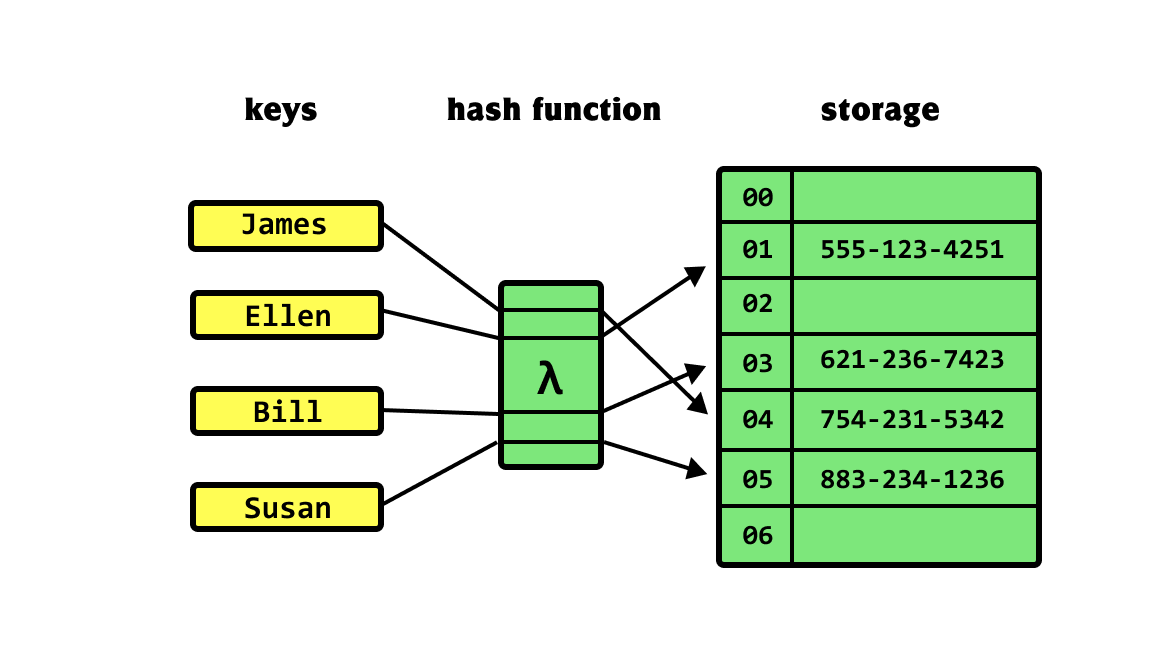
\includegraphics[width=9cm, height=4cm]{Figure4.png}}
\caption{Hashing Example}
\label{fig4}
\end{figure}

\smallskip
\noindent
\textbf{Hashing:} The hash key in a data vault hub is used to improve the lookup performance within a data warehouse \cite{b5}. This comes in handy when querying the final Data Vault model which necessitates many more joins than querying a typical database. In addition to performance, hashing ``Fig.~\ref{fig4}'' provides a layer of security. hash keys are calculated with the MD5 algorithm.

\begin{figure}[htbp]
\centerline{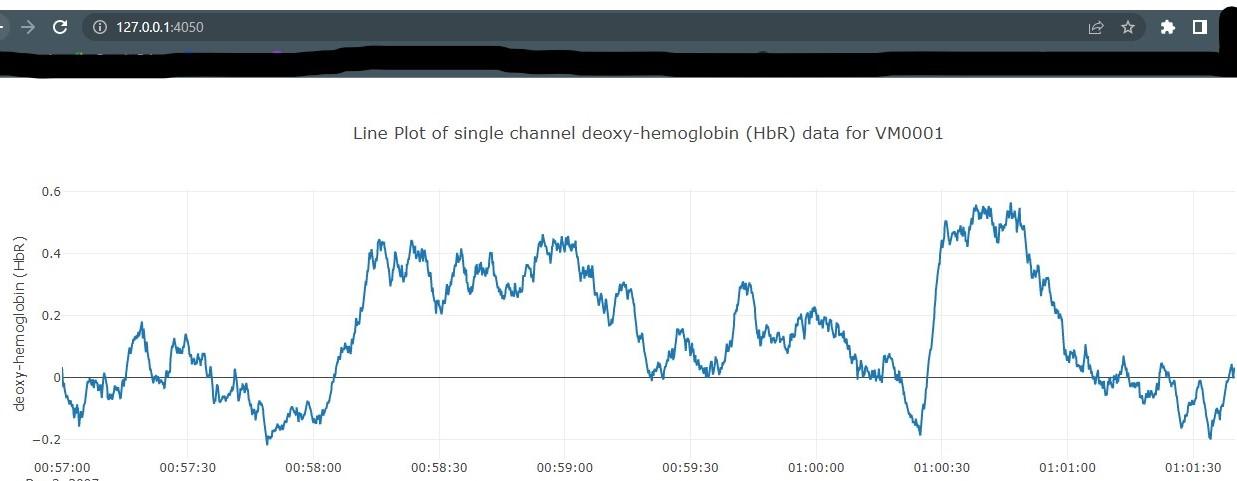
\includegraphics[width=9cm, height=4cm]{Figure5.png}}
\caption{Browser based GUI Interface Example}
\label{fig5}
\end{figure}

Dimensional modeling, often known as Kimball's star schema is used to build information marts. Star schema has two types of tables, fact table and dimension table. Fact tables include information about certain business processes or events that occur inside these processes. They provide reference to each dimension. Fact tables may also contain measure which are numerical quantifiable values. Dimensions gives meaning when joined with fact Tables. They are critical to the data warehouse's understanding as all descriptive information is taken from the dimension tables. They can also be used to filter facts based on the dimensions themselves or one of their descriptive qualities. 

Additionally, aggregated measurements can be sorted by dimension or one of its properties. Providing facts and dimensions using virtualized approaches is more agile and responsive to user requests than ETL-based integration. These approaches require no data
moving or data materialization and are far easier to design and develop \cite{b6}. A browser based intuitive GUI ``Fig.~\ref{fig5}'' for querying is implemented using plotly that receives data from virtualized information marts and visualized them using graphs and charts accessible to users unfamiliar with querying.


\section{Results}

Metadata from the raw data is extracted from raw files and added to a dictionary variable, metadata ``Fig.~\ref{fig6}'' can comprise various datatypes that need to be extracted. To preserve the data types, data is loaded in postgres using a binary stream and encoded. Maintaining the object datatypes allows us to operate on them during the data retrieval stage. Data values are followed by metadata, they are retrieved in a structural format using libraries that read data in tabular format such as pandas.

\begin{figure}[htbp]
\centerline{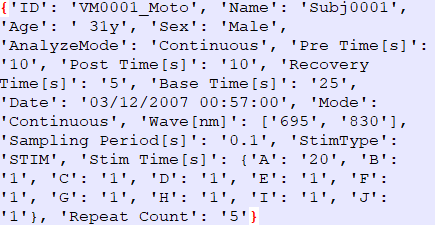
\includegraphics[width=9cm, height=4cm]{Figure6.png}}
\caption{Sample metadata Extraction in text format}
\label{fig6}
\end{figure}


Satellite tables contain a part of descriptive information, while Hubs ``Fig.~\ref{fig7}'' connect the satellites ``Fig.~\ref{fig8}'' and in turn, multiple hubs are connected by links ``Fig.~\ref{fig9}''.

\begin{figure}[htbp]
\centerline{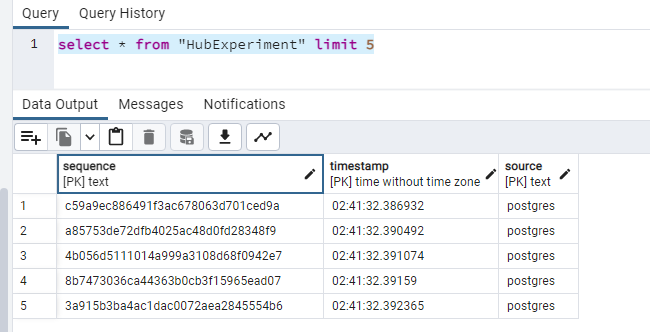
\includegraphics[width=9cm, height=4cm]{Figure7.png}}
\caption{Hub Data Example}
\label{fig7}
\end{figure}

\begin{figure}[htbp]
\centerline{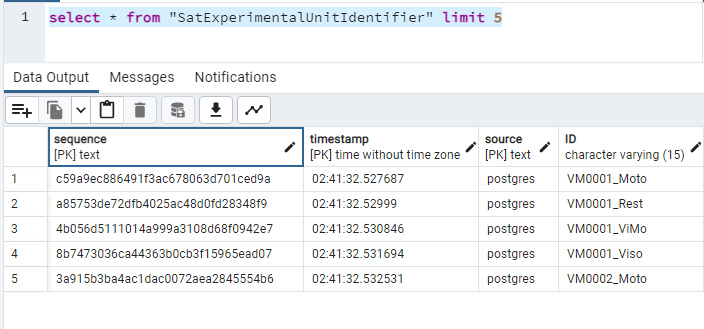
\includegraphics[width=9cm, height=4cm]{Figure8.png}}
\caption{Satellite Data Example}
\label{fig8}
\end{figure}

\begin{figure}[htbp]
\centerline{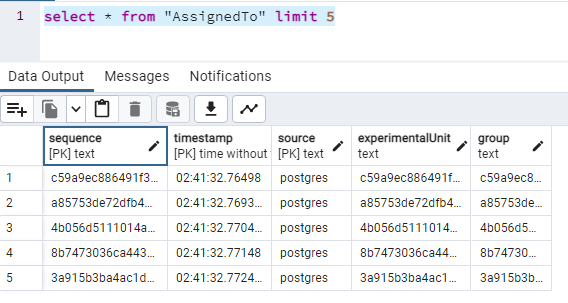
\includegraphics[width=9cm, height=4cm]{Figure9.png}}
\caption{Link Data Example}
\label{fig9}
\end{figure}

The data from the enterprise data vault are consumed by information marts, each piece of information serves a business purpose and is characterized by fact and dimension tables described earlier. These are virtualised in the form of views ``Fig.~\ref{fig10}''.

\begin{figure}[htbp]
\centerline{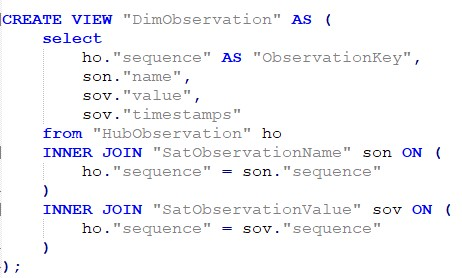
\includegraphics[width=9cm, height=4cm]{Figure10.png}}
\caption{Sample Dimension View}
\label{fig10}
\end{figure}

Final layer will be GUI that consumes data from Information mart and visualizes them in graphical ``Fig.~\ref{fig11}'' form. In this section the user has the ability to choose the data he needs to view. Drop-down options are provided to browse a particular experiment.


\begin{figure}[htbp]
\centerline{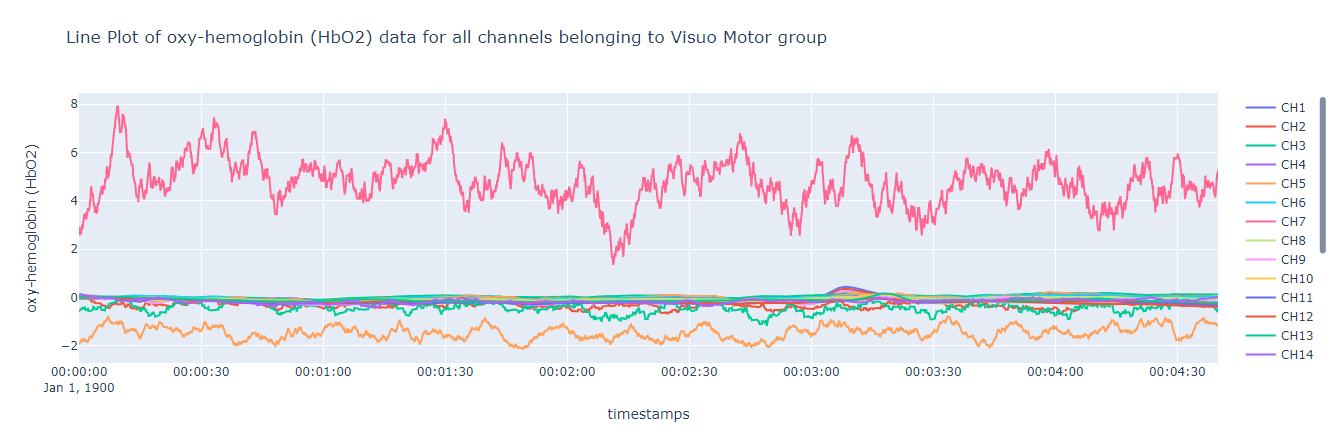
\includegraphics[width=9cm, height=4cm]{Figure11.png}}
\caption{Example Graphical GUI charts}
\label{fig11}
\end{figure}

\section{Discussion}

Data vault provides the flexibility to start small and overtime expand the resources. The enterprise layer need not be designed completely in one go. A specific domain requirement that has priority could take up as a modular part. Hubs, Satellites and links are built. An Information Mart of this specific domain is created and insights are derived from Information Mart from limited domains. As the requirement increases further, Data Vault will be scaled up to add new domains and serve a different use case. It provides us the ability for a continuous development life-cycle with regular deliverables added and supported in an \textbf{agile} way.

Data Vault overcomes the limitations posed by older models by Inmon and Kimball. Compared to Inmon model, which increases complexity with the increase in requirements, data vault address this in the form of Hub and Satellite architecture which reduces complexity by separating each of the domains. Similarly, compared to Kimball architecture, where update anomaly poses a challenge, data vault mitigates it by just providing data insert options and eliminating updates.

The modeling style is a unique combination of third normal form and dimensional modelling approaches to fulfil the demands of enterprise. The design pattern allows the data vault to offer scale-free characteristics, which means that there are no intrinsic constraints on the size of the model or the quantity of the data that model represents, other than those imposed by the infrastructure \cite{b7}. To add new areas, it scales horizontally, while the scaling is vertical when huge data of same business utility gets added to the model.

\section{Conclusions}

Building a data vault needs specific skills to master for having an efficient model. The learning curve to design the vault needs specialist who segregated and decide where the data needs to reside, have the ability to design hubs, satellites and links, and develop an understanding to choose business keys that reflects and defines the business object in the whole warehouse.

Data vault provides an advantage when the requirements have high scalability, and need an agile approach with enhanced security features. Data vaults also have an enhanced query performance with security due to hashing implementations for business keys. Data vault allows for faster data ingestion with audit as multiple tables can be loaded simultaneously from varying source systems without bottlenecks. Data Vaults also provide flexibility to serve multiple applications. Adding a new domain is as simple as creating a new Hub with satellites to store information avoiding remodeling the existing structure in place. This also serves when an organisation decides to expand the data vault to add new domains.

\begin{thebibliography}{00}
\bibitem{b1} Daniel Linstedt, Michael Olschimke, "Building a Scalable Data Warehouse with Data Vault 2.0", 2016, pp 89-121, ISBN 9780128025109.
\bibitem{b2} L. Yessad and A. Labiod, "Comparative study of data warehouses modeling approaches: Inmon, Kimball and Data Vault," 2016 International Conference on System Reliability and Science (ICSRS), 2016, pp. 95-99, doi: 10.1109/ICSRS.2016.7815845.
\bibitem{b3} L. Yessad and A. Labiod, "Comparative study of data warehouses modeling approaches: Inmon, Kimball and Data Vault," 2016 International Conference on System Reliability and Science (ICSRS), 2016, pp. 95-99, doi: 10.1109/ICSRS.2016.7815845.
\bibitem{b4} Daniel Linstedt, Michael Olschimke, "Building a Scalable Data Warehouse with Data Vault 2.0", 2016,Chapter 4 - "DATA VAULT 2.0 MODELING", pp 97, ISBN 9780128025109.
\bibitem{b5} Daniel Linstedt, Michael Olschimke, "Building a Scalable Data Warehouse with Data Vault 2.0", 2016,Chapter 4 - "DATA VAULT 2.0 MODELING", pp 98, ISBN 9780128025109.
\bibitem{b6} Daniel Linstedt, Michael Olschimke, "Building a Scalable Data Warehouse with Data Vault 2.0", 2016,Chapter 14 - "LOADING THE DIMENSIONAL INFORMATION MART", pp 585, ISBN 9780128025109.
\bibitem{b7} Inmon, W.H.H. and Linstedt, D., 2014. Data architecture: a primer for the data scientist: big data, data warehouse and data vault. Morgan Kaufmann.
\end{thebibliography}


\end{document}